%# -*- coding: utf-8-unix -*-

\chapter{机票推荐中的冷启动问题}
\label{chap:cold}

冷启动问题一般分为物品冷启动和用户冷启动。前者的含义是当一件物品新添加到物品库中,在还没有用户使用过的情况下如何将其推荐给用户;后者的含义是当一名新用户来到推荐系统,在完全没有用户偏好的情况下如何为用户推荐适当的物品。冷启动问题是推荐系统需要面对的严峻问题。如果处理不好冷启动问题,系统内添加的新物品可能永远都无法向用户推荐;也会影响到新用户的体验,造成用户流失。\par
在机票推荐系统中,由于机票的数量非常有限并且每条航线上的航班较为固定,通常不会面临物品冷启动问题。而机票本身属于低频、刚需物品。因此机票推荐系统面临的主要问题是用户冷启动问题。在传统的推荐系统中,有一些办法可以解决用户冷启动问题:如在电子商务、书籍网站,用户往往会先提供物品的类别、品牌等信息,随后可以将类别下购买人数的商品推荐给新用户;而在视频、新闻等内容网站,可以在新用户注册时让用户勾选一些感兴趣的主题,即使没有有效获取用户的偏好主题,仍可以将总体最热门的、最实时的内容呈现给用户。\par
在机票推荐研究领域,由于其业务的特殊性,这两种做法均有不足之处。由于机票具有动态属性,难以静态地描述;并且每个航班的机票数量最多在一两百左右,造成的结果是热门物品与冷门物品之间的差别很小。因此很难单纯以热门程度进行推荐。在第三章,图\ref{fig:res_pref_rec}中的结果表明,以航班热门程度排序的策略难以表现出好的推荐效果。其次,影响用户购买决策的因素有很多,用户每次选购机票时注重的属性可能会因为用户的日程安排、出行目的的不同而发生变动。而在内容网站,用户的兴趣主题一般不会发生频繁变动。\par
在第三章中,图\ref{fig:user_user_percent}的统计结果表明,在北京-上海这条热门程度很高并且订单、用户数量比最高的航线上,平均每位用户的订单数量仅为两单,仍有$60\%$的用户在过去两年仅订过一单,$90\%$的用户仅订过不多于四单。订单数量在四单及以下的用户占了订单总数的$60\%$。在机票票务服务业务领域,用户冷启动现象也严重影响到用户体验及机票推荐效果。因此需要对冷启动问题展开深入研究。


\section{航线分析及推荐差异}
本小节我们主要对机票推荐中冷启动问题对推荐结果带来的负面影响进行分析与阐述。此处我们仍然选取第三章中提到的四条热门航线进行分析。

\subsection{航线特征分布及用户行为分析}

我们在第三章中提出的机票推荐算法首先将用户数据按照航线进行分割。并为每个用户在每条他选购过机票的航线上独立维护一个特征分布模型。这样的做法细化了推荐粒度,使用与目标推荐航线相同的航线来进行建模可以得到更贴合的用户偏好。但是用户的历史订单数据却分散到各个航线。如果在待推荐航线上的训练数据过少,则难以精确刻画用户的偏好。在此我们首先分析航线间的差异;并分析按航线为用户提取偏好对推荐效果带来的影响。

\begin{figure}
\centering
\subfigure[北京-上海航线价格等级分布图]{
 \label{fig:sha-pr}
 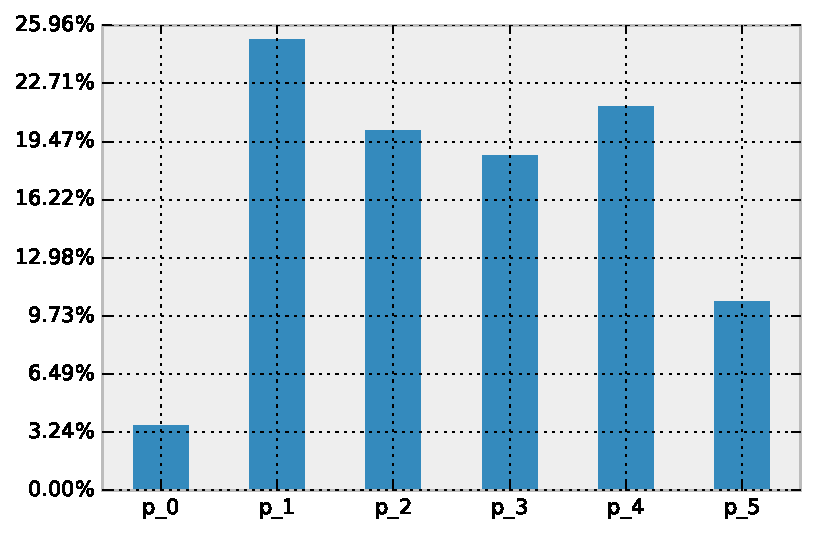
\includegraphics[width=0.49\linewidth]{06/3_pr_dis_bjs.pdf}}
\subfigure[北京-西安航线价格等级分布图]{
 \label{fig:xiy-pr}
 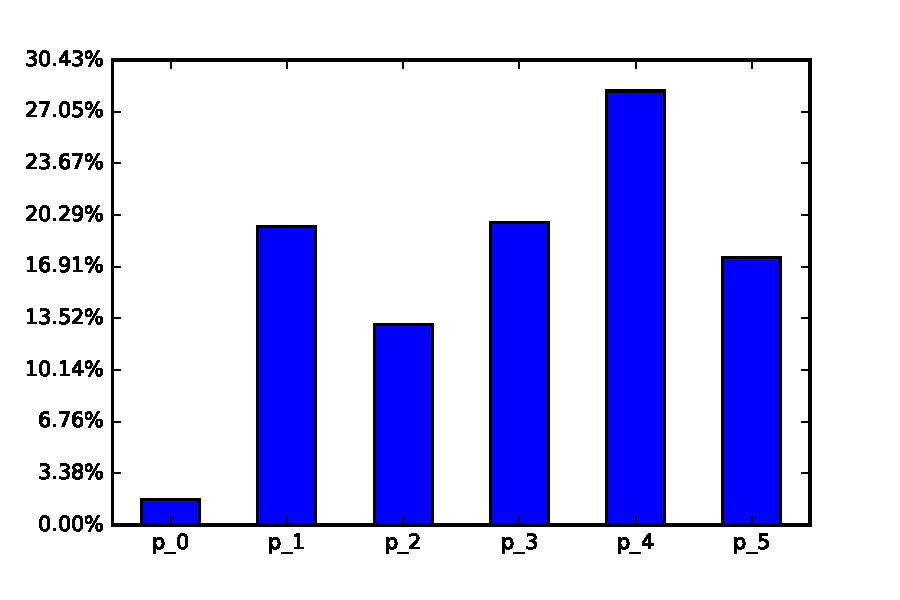
\includegraphics[width=0.49\linewidth]{06/4_pr_dis_xiy.pdf}}
\bicaption[fig:pr_dis]{价格等级分布}{航线间价格指数分布差异}{Fig}{Figure for Variety of  Price Range}
\end{figure}\par

图\ref{fig:sha-pr}展示了北京到上海航线上的价格指数的分布情况,其横轴的各个标签代表不同的价格指数等级,根据前文提出的价格指数概念,我们将价格指数按照增序划分到$P_0 ~ P_5$六个等级,机票订单价格逐级下降;其纵轴代表位于该价格等级的订单占订单总量的百分比;类似地,图\ref{fig:xiy-pr}展示了北京到西安航线的价格指数分布情况;两图对比可以看出,两条热门航线上价格指数等级的分布占比既有相似之处,也有部分差异。相似之处在于:价格位于最高区间的机票订单数量最少,价格位于最低区间的订单量也较少,而大部分订单集中在中间的价格区间;差异之处在于:在北京到上海航线,高价格区间的订单总体数量占比较大,
其中$P_1$区间的订单总量最多,达到$25\%$;而在北京到西安的航线,低价订单的总体占比较大,
$P_4$区间的订单总量最多。这也与我们之前结合订单、用户数量比得出的航线间出行目的差异相吻合。根据上图的分析我们可以发现,不同航线上的特征分布有所不同。

\begin{figure}
\centering
\subfigure[北京-上海航线航司标准熵分布图]{
 \label{fig:sha-h}
 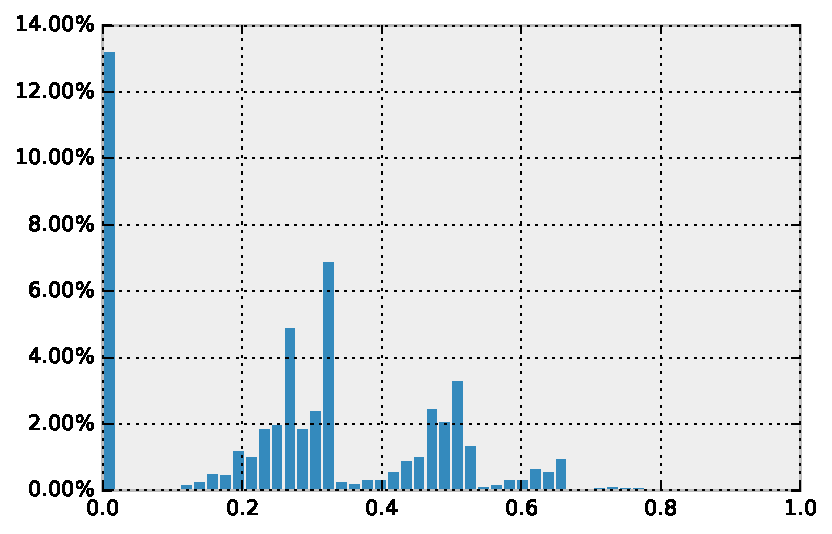
\includegraphics[width=0.49\linewidth]{06/1_entropy_airline_sha.pdf}}
\subfigure[北京-西安航线航司标准熵分布图]{
 \label{fig:xiy-h}
 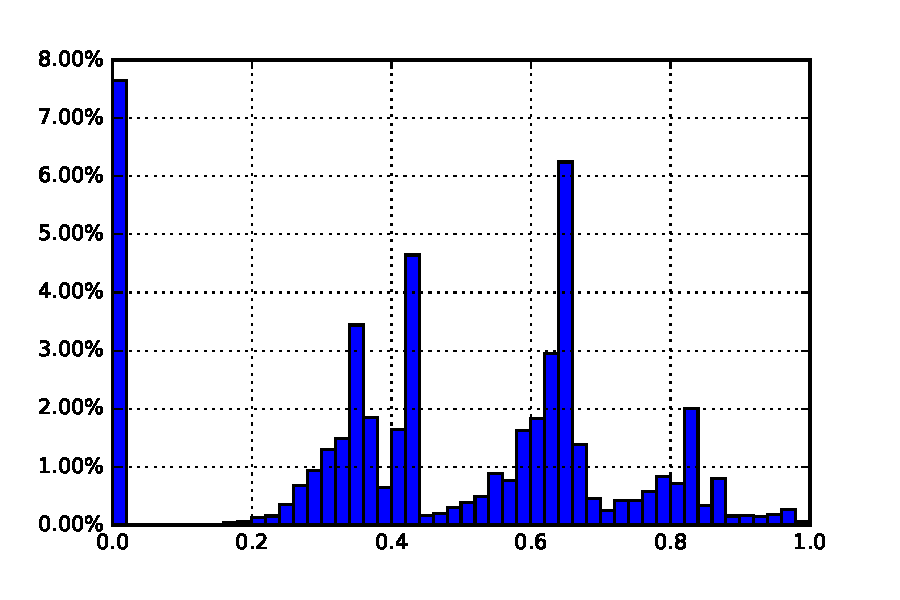
\includegraphics[width=0.49\linewidth]{06/2_entropy_airline_xiy.pdf}}
\bicaption[fig:h_dis]{标准熵分布}{航线间标准熵分布差异}{Fig}{Figure for Entropy Variety of Airline}
\end{figure}\par
图\ref{fig:sha-h}和图\ref{fig:xiy-h}分别展示了北京到上海航线和北京到西安航线的航司标准熵分布图,横轴代表标准熵值,
是将根据公式\ref{eq:entropy}计算出的熵值除以向量的维度进行归一化得到的值。其取值范围在$[0,1]$,用户的偏好集中程度随着熵值的减小而增加。纵轴代表用户的数量占比,即航司偏好的标准熵在该值的用户占用户总数的比例。两条航线都是在标准熵小于0.02的用户数量最多;北京到上海航线上,有更多比例的用户在航司维度的标准熵小于0.02,并且整体熵值偏小,证明在该航线上,用户对航司的偏好更集中。而北京到西安航线,更多的用户集中在0.6附近,相比于前者,用户在该航线上的对航司的偏好更加分散。\par

至此,我们根据图\ref{fig:pr_dis}反映了不同航线上总体特征分布的差异,这是航线之间客观存在的差异,可能与航空公司的定价策略及票源供给策略等挂钩。还根据图\ref{fig:h_dis}分析了不同航线上用户偏好集中程度的差异,这属于用户主观行为的差异,会受到航线的属性、起飞城市和落地城市的社会性质等因素影响。我们分析对比了客观、主观两个方面的因素对航线造成的影响,也因此造成了航线间的差异。

\subsection{航线差异对机票推荐造成的影响}

分析了航线特征分布及用户偏好集中程度的差异后,需要研究航线间差异对推荐效果的影响。我们的基本思路是分别使用与推荐航线不同航线的特征分布模型为用户进行机票推荐,并评估推荐效果。如果使用不同航线上的用户特征分布模型的推荐效果相差不多,则证明航线差异不影响机票推荐;反之则证明航线差异对推荐结果的影响不可忽视。

\begin{figure}
 \centering
 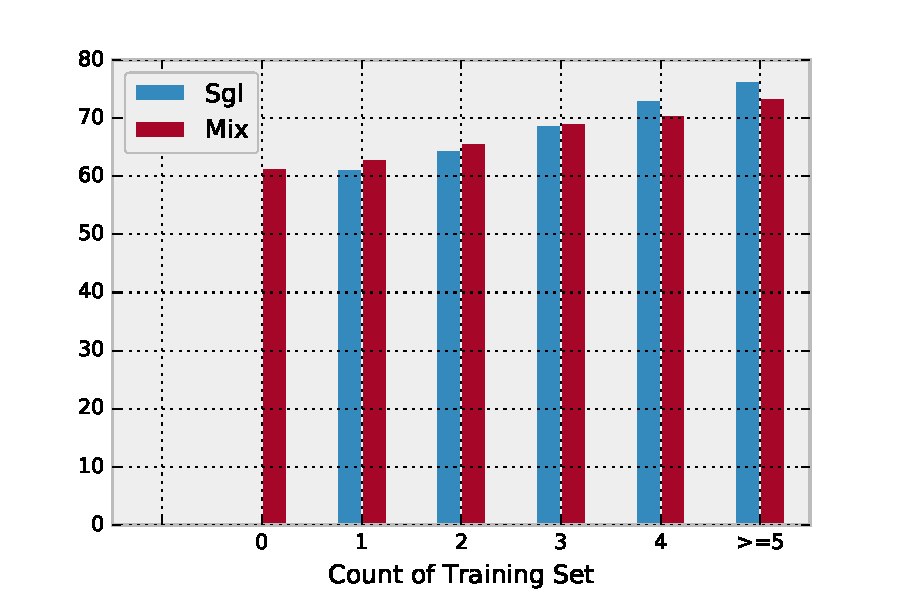
\includegraphics[width=0.9\linewidth]{06/5_res_of_sgl_mix.pdf}
 \bicaption[fig:slg_mix_rec]{航线推荐效果对比}{单一航线与混合航线的推荐效果对比}{Fig}{Accuracy of Recommendation for Single and Mixure Airline}
\end{figure}\par

图\ref{fig:slg_mix_rec}展示了在北京到上海航线上分别仅使用目标航线特征分布模型(Sgl,以下称为单一航线模型)以及
使用混合航线特征分布模型(Mix)进行机票推荐的效果。为了获取有效推荐结果,必须抽取出一条订单作为测试订单,我们将测试订单所在航线定义为目标航线,用户在该航线上其他订单定义为训练订单。对于单一航线模型推荐算法,我们无法为在该航线上只有一条订单的用户进行推荐结果验证。
这里混合航线模型的含义是直接使用用户在所有航线(包括目标航线)上的历史订单作为训练订单。图的横轴代表用户在目标航线的训练订单条数。纵轴代表推荐平均准确率。对于单一航线模型的推荐算法,其训练订单的数量等于横轴标注的数量;而对于混合航线模型推荐算法,训练订单还要再加上用户在其他航线上的历史订单,数目不确定。但在我们要解决的问题中,用户的订单量普遍较为稀少,所以混合模型中的总训练订单数量一般不会太大。\par
从图中我们可以看出,当目标航线训练订单数量为三条及以下时,使用混合航线模型的推荐效果好于单一航线模型。两者之间的差距随着订单数量的增加而减小。当目标航线上的训练订单数达到三条时,两种模型的推荐效果没有明显差异,但单一航线模型的计算开销和数据吞吐开销都较小。当训练订单多于四条时,使用单一航线模型的推荐效果好于混合航线模型。由此我们可以得出结论,在用户建模时使用的数据不一定越多越好,由于航线差异可能导致其他航线的特征分布模型稀释了用户在目标航线上的偏好。为用户按照航线区分特征分布模型对于订单数量在三单以上的用户具有较好的推荐效果。
从图中还可以发现,当目标航线没有训练订单时,混合航线模型的机票推荐结果也相当不错,与只有一单训练订单时的单一航线模型推荐结果相差无几。可以说明当用户的订单量较少时,学习的特征分布模型具有一定的偶然性。并且用户在其他航线上的偏好具备一定程度上的借鉴意义。在实际生产环境中,我们没有测试订单、训练订单的概念,为了兼顾系统性能与用户体验,可以直接使用该用户在其他航线上的数据进行偏好建模。

\section{基于社会关系解决用户冷启动问题}

\subsection{特征权重训练}

多人时间衰减、训练权重



\section{航线冷启动问题的分析}
前文我们分析了航线间差异及对个性化机票推荐带来的影响。本节我们针对航线冷启动问题进行研究。航线冷启动问题的含义是用户在需要进行推荐的目标航线上没有历史订单或订单数量较少。根据前文的对照实验结果,我们主要针对的用户是用于建模的目标航线训练订单数量少于三单的用户。

\subsection{航线间差异的量化}

这类用户由于订单量较少,无法在目标航线建立精确的特征分布模型,但在其他航线具有部分订单。为了针对这批用户解决航线冷启动问题,一个基础的思路是我们需要将用户在其他航线上的特征分布模型进行适当的修正,使其能够克服航线间的差异,以符合用户在目标航线上的偏好。为此,我们首先需要能够量化航线间的差异程度。\par
我们仍使用相似度函数来分析航线间的差异。对于结构化的物品。我们可以对其进行特征提取,则物品可以由同构的特征-取值键值对表示。在衡量物品的整体相似度时,可以先按照每个特征的内容组成衡量局部相似度,再将个局部相似度进行融合,就可以得到整体相似度。相似度融合的策略一般是以特征在整体中的相对重要程度定义一个权重指数。因此,整体相似度的衡量公式可以定义为:
\begin{equation}
	Sim(A,B) = \sum_{f \in F}w(f) \times \sigma(f)
\end{equation}\par
$w_f$代表特征权重。$\sigma_f$是特征局部相似度衡量方法。为机票进行相似度衡量时,机票的每一个特征对应具体数值,我们需要为每个特征所有可能的取值之间定义相似度分数,往往需要借鉴业务领域知识。在航线相似度衡量中,我们可以从与机票类似的角度出发,将航线以多维度特征表示。航线的关键特征与前文提到的特征一致,包括价格、起飞时间、机型、舱位等级、航司和退改签政策。与机票不同的是,航线上的每个特征包含所用用户订单。这里,我们使用航线在每个特征的总体分布向量来代表该航线的对应特征。此外,我们在之前的章节展示了不同航线在用户行为方面有一定的差异,表现在该特征的用户标准熵的分布有较大
差异。因此,用户行为也作为我们衡量航线相似度的一个考虑因素。\par
航线每个特征的分布可以表示为向量,每个向量所有维度的取值之和为1。我们对特征使用同样的离散化策略。对于航司特征,其种类多达数十种,而每条航线上出现的航司组合不尽相同,往往只有不到十种。如果将所有的航司都罗列到一个向量中,则大多数维度的分布百分比都是0,会对相似度的衡量带来干扰。因此,我们使用字典来维护这个特征。在衡量两条航线在航司的相似度时,我们首先将各自的字典进行扩容,使它们的键包含两条航线上航空公司的并集,可以将航司特征也转化为向量。这里我们使用欧几里德距离作为衡量航线在一个特征上分布差异的公式:
\begin{equation}
	Dist(\mathbf{X},\mathbf{Y}) = \sqrt{\sum_{i=1}^{|X|}(x_i-y_i)^2}
\end{equation}
\begin{equation}
\label{eq:a_sim}
	DistSim(\mathbf{X},\mathbf{Y}) = \frac{1}{Dist(\mathbf{X},\mathbf{Y})}
\end{equation}\par
欧氏距离衡量了两个向量在空间上的距离,适合在两个相同维度以及量纲的向量之间进行比较。在公式中,$\mathbf{X}, \mathbf{Y}$代表需要计算相似度的向量。式\ref{eq:a_sim}定义了以欧式距离为基础的相似度衡量公式,可以得出当两个向量的欧氏距离为0时,它们的相似度为$1$,且随着欧式距离的增加,向量间相似度递减。
对于用户行为相似度的衡量,结合上一节我们统计过用户熵值分布百分比,我们可以将标准熵在$[0,1]$取值区间内均匀划分为$50$个区间,将每个区间视作一个维度,
将用户熵值在一个特征上的分布也转化为向量,记作$S(f)$。
下公式给出结合航线分布和用户行为的航线间特征相似度衡量方法:
\begin{equation}
	\sigma(f) = DistSim(\mathbf{f_a,f_b}) + DistSim(S(\mathbf{f_a}),S(\mathbf{f_b}))
\end{equation}\par
$f_a, f_b$是待比较航线上的一个特征,第一项代表航线间特征分布的相似度,第二项代表在该特征上用户行为分布的相似度。每个特征的权重定义为两条航线上该特征分布的标准熵之和。
\begin{equation}
	\overline{S}(\mathbf{f_a}) = \frac{\ln |f| - S(\mathbf{f_a})}{\ln |f|}
\end{equation}
\begin{equation}
	w(f) = \overline{S}(\mathbf{f_a}) + \overline{S}(\mathbf{f_b})
\end{equation}\par
计算出两条航线在所有特征的权重后,将所有值进行归一化就得到了标准权重。至此,我们从特征分布和用户行为两个方面量化了航线间的差异。在解决航线冷启动问题时,可以根据这个量化方法,对用户在非目标航线的特征分布模型进行修正,进而将其应用在机票推荐中。

\subsection{最优航线的选取及模型修正}
本小节主要介绍我们如何根据航线间差异量化方法为航线冷启动用户选取最优非目标航线并进行模型修正。一个最简单的方法是从用户订单中选出与目标航线差异度最小的航线,将用户在该航线的特征分布模型应用在目标航线。这种做法存在几个问题。首先,用户可能在与目标航线相似度最高的航线上也属于冷启动跃用户,这条航线虽然最符合我们的策略,用户在其上的特征分布模型也具备相当大的偶然性,因而对提升推荐效果起不到显著作用;其次,虽然选出了与目标航线差异最小的航线,并且用户有足够多的订单,但用户在那条航线上的模型也与该航线的整体特征分布有密切联系,因而无法直接使用在目标航线的推荐中。\par
鉴于以上几点,我们首先需要选取合适的非目标航线,还要对用户在该航线的特征分布模型进行修正。为了避免第一个问题,我们在与目标航线相似度的基础上加上用户在本航线的订单数量作为一个激励因子,将航线相似度和订单数量都作为度量因素,提出了加权相似度公式:

\begin{eqnarray}
\label{eq:rsim}
	ReSim(\mathbf{R_a,R_b}) & = & \log{|O_b|} * Sim(\mathbf{R_a,R_b})  \nonumber \\
                        & = & \log{|O_b|} * \sum_{f \in F}w(f) \times \sigma(f)
\end{eqnarray}\par

式\ref{eq:rsim}在原本相似度公式的基础上添加激励因子,公式中$R_a$代表目标航线,$R_b$代表候选航线,$O_b$代表在候选航线上的订单,我们需要为用户滤掉订单数量不超过一条的航线。在激励因子项我们取订单数量以10为底的对数,避免订单数量对航线相似性的度量造成过大影响。在选取最优航线时,我们将所有非目标航线按照与目标航线的加权相似度进行排序,取出最相似的航线用作模型修正。\par

模型修正

皮尔逊相关系数 分析偏好与航线分布的关系



\subsection{实验结果分析}

相似度表格,相关系数表格,推荐结果(全航线作对照)